\section{Offline Synthesis and Repair Case Study}
\begin{figure}
    \centering
    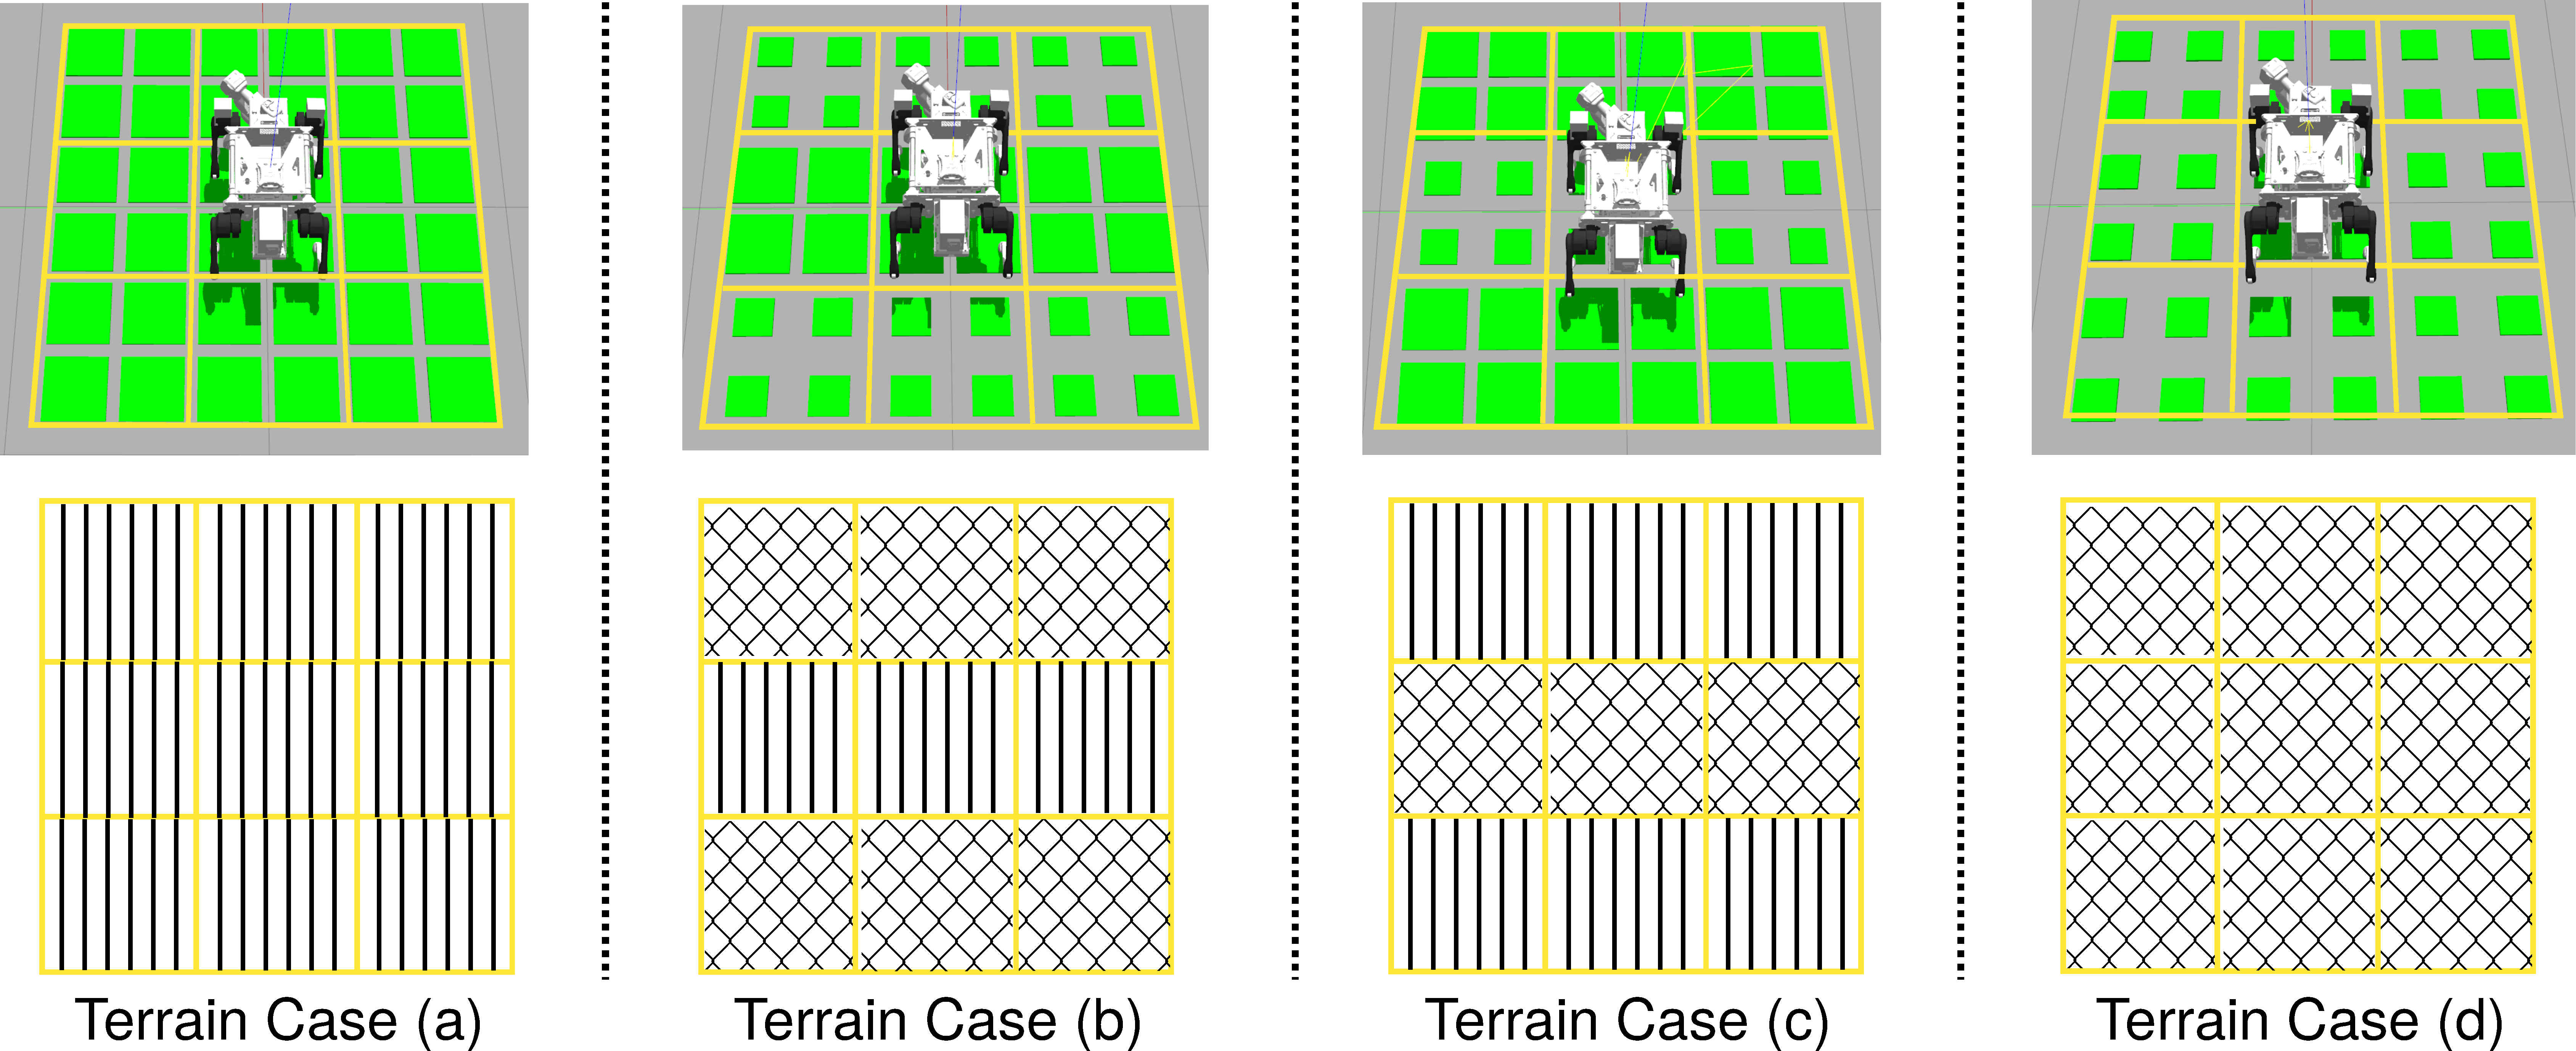
\includegraphics[width=1\linewidth]{offline_terrains.pdf}
    \caption{Four terrain cases used for offline repair in our case study.}
    \label{fig:offline_terrains}
\end{figure}
\begin{figure}
    \centering
    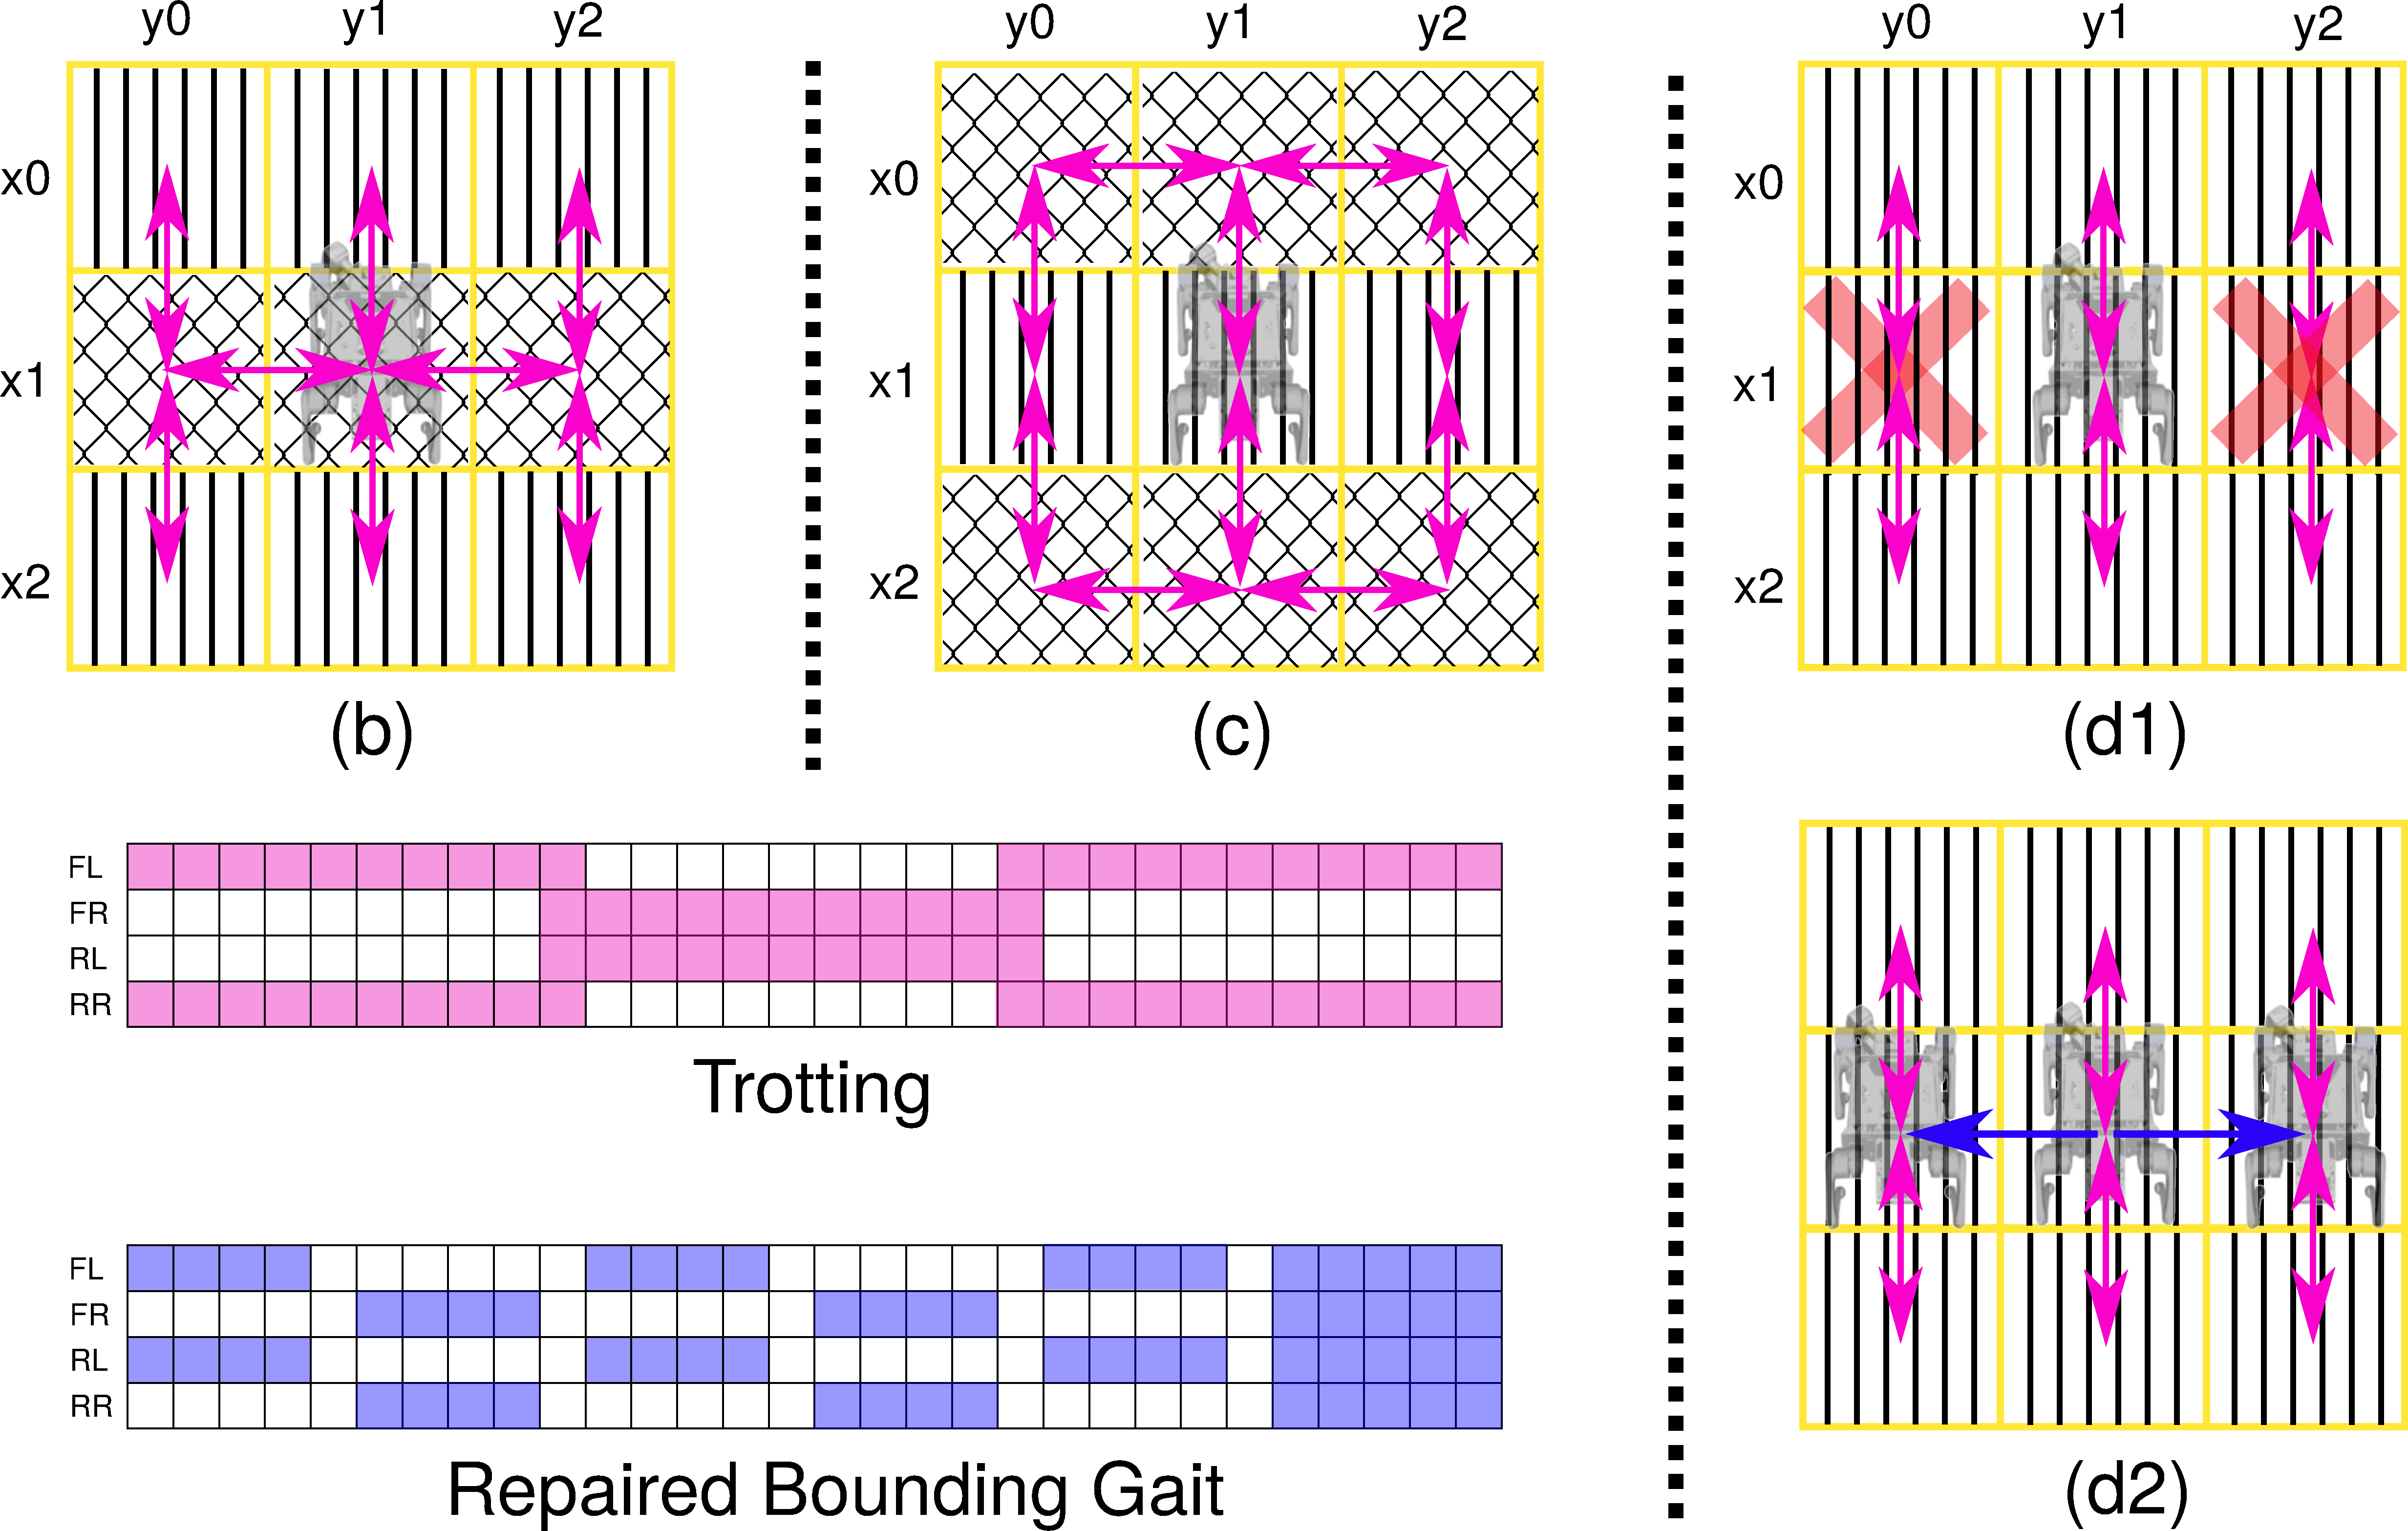
\includegraphics[width=\linewidth]{offline_repair.pdf}
    \caption{Offline repair results for terrain cases (b), (c), and (d) in Fig.~\ref{fig:offline_terrains}. We also illustrate the original trotting and repaired bounding gait.}
    \label{fig:offline_repair}
\end{figure}
We first present a case study to demonstrate the synthesis and repair processes in offline phase. 
% \subsection{Offline Synthesis and Repair Case Study}
Complementary to Example~\ref{example:1}, we provide additional set of predefined terrain polygons, which are abstracted into sparse and dense terrain types similar to Example~\ref{example:1}.
Fig.~\ref{fig:offline_terrains} shows four 9-grid terrain combinations with varying stepping stone sparsities. The first row presents the real-world terrain polygons, while the second row displays the corresponding symbolic-level maps. The grid size is chosen based on factors such as robot size and terrain dimensions. In this case study, we use a 0.6 m cell size and a $1.5$ s trotting gait as the motion primitive given ahead of time, and the MICP planner has a $0.02$ s timestep, resulting in $N=75$ knot points, and $R=8$ terrain polygons per transition. 

In Fig.~\ref{fig:offline_repair}, the pink arrows indicate the original feasible transitions after performing the gait-fixed MICP. The robot successfully navigates upward and downward across all terrains; terrain case (a) achieves all transitions and is not shown in the figure due to space limit. 
The infeasible transition arises when moving sideways on sparse stepping stones, restricted by the leg kinematics constraint in Eq.~\ref{eq:rom}. However, specifications for terrain case (b) and (c) remain realizable as the robot avoids sideways movement by taking detour steps, indicating that not all skills are required for these types of  terrains. Such a coincidence does not apply to terrain case (d), where the specification becomes unrealizable due to physically unreachable $(x_1,y_0)$ and $(x_1,y_2)$. This unrealizability triggers a symbolic repair to identify a symbolic suggestion, adding two additional transitions (blue arrows). By reconfiguring to a bounding gait with short aerial phases through gait-free MICP, the robot restores transition feasibility, making terrain case (d)'s specification realizable.

% we the offline terrains for specification generation. We use the above case for demonstrating the offline repair. We can emphasize that not all the transitions are needed for navigating to a desired waypoint considering the robot physical feasibility. The robot does not necessarily need to move sideways. It becomes more urgently needed when the state space increases. This also allows us to incorporate strategy in terms of specific terrain combinations. Only exception case is the one with all sparse terrains.

